\documentclass{standalone}
\usepackage{standalone}

\begin{document}

\section{Overview}
We separate our process into several stages. Each stages contains several steps in it. An overview of all stags in our process is shown in Figure \ref{fig:ProcessOverview}. The process will be described in more details in the following sections.

\begin{figure} 
	\centering
	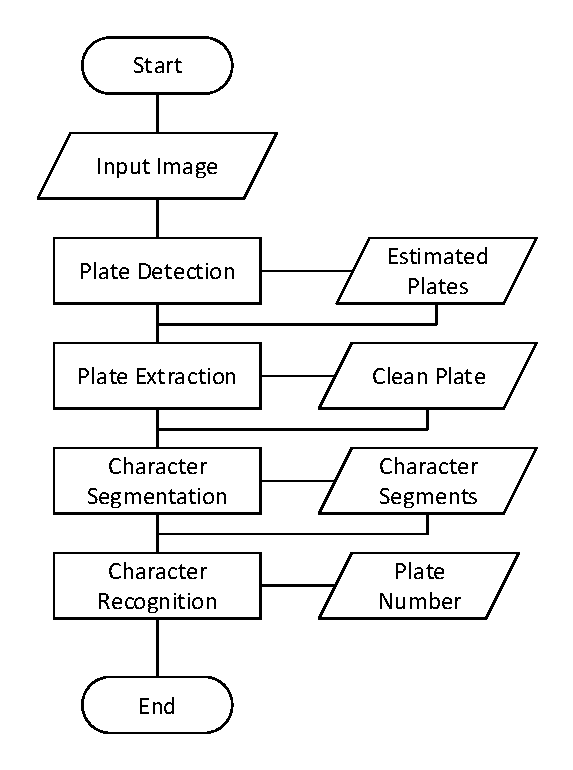
\includegraphics[width=0.8\linewidth]{./img/plots/overview}
	\caption{An overview of the plate detection procedure.} 
	\label{fig:ProcessOverview}
\end{figure}

\begin{description}
\item [Input Image] is a 24-bit colored image with red, green and blue channels.
\item [Preprocessing] stage applies several operations on input image to convert it into an image suitable for feature analysis for later stages. In our case, it also outputs general location of the plate.
\item [Plate Detection] analyses all plate like locations, and extract plates from them. Also it cleans the plate for segmentation.
\item [Segmentation] step is for splitting the characters from the plate. It is done so that the characters can be recognized by the OCR.
\item [Plate recognition] uses an OCR system to recognize individual characters and text images.
\end{description}

\end{document}